\documentclass[10pt]{article}
% arXiv submission: declare PDF output (their pipeline defaults to DVI otherwise)
\pdfoutput=1
\usepackage[margin=1in]{geometry}
\usepackage[utf8]{inputenc}
\usepackage[T1]{fontenc}
\usepackage{lmodern}  % scalable Type1: required for T1 + microtype on arXiv
\usepackage{amsmath,amssymb,amsfonts}
\usepackage{graphicx}
\usepackage{booktabs}
\usepackage{multirow}
\usepackage{xcolor}
\usepackage{tikz}
\usetikzlibrary{shapes.geometric,arrows.meta,positioning,fit,calc}
\usepackage[numbers,sort&compress]{natbib}
\usepackage{microtype}
\usepackage[hidelinks,pdftitle={Cache Translation Across Model Scale: An Audit with Identity Controls and Oracle Probes},pdfauthor={Anonymous}]{hyperref}

\newcommand{\kv}{\mathrm{KV}}
\newcommand{\chg}{\mathrm{CHG}}
\newcommand{\gold}{p_{\mathrm{gold}}}

\title{Cache Translation Across Model Scale:\\
An Audit with Identity Controls and Oracle Probes}

\author{}
\date{}
\date{}

\begin{document}
\maketitle

\begin{abstract}
Cache translation maps the key-value (KV) cache that a large teacher model
forms over a context into the cache space of a smaller student model, so that
the student answers without re-prefilling the context. A growing line of work
reports quality-preserving translation across heterogeneous models. We audit
this claim on Qwen3 pairs (8B$\to$1.7B, 8B$\to$0.6B, 4B$\to$1.7B, and 4B$\to$0.6B), plus five cross-architecture students, with a three-hypothesis
framework and two instruments that prior evaluations omit. First, an
\emph{identity control} injects the student's own cache through the full
translation-and-injection pipeline: it reproduces the student's own prefill
exactly (per-sample logit cosine $1.000$), which isolates mechanics from
mapping. Second, \emph{oracle probes} mix teacher-cache content into the
student's own cache and probe what the student can extract from
translated content. Across seven
mapper families (per-head ridge, affine, per-layer affine, task-aware, a
residual-anchored translator, a per-head MLP, and an over-parameterized
joint MLP), a controlled calibration
ladder on a fixed evaluation set, and 96 recorded audit-protocol runs, no configuration
makes the strong student exceed its own prefill: gold-probability change
spans $-0.14$ to $-0.39$ against a self-kv control at $+0.000$. Calibration
budget is inert (CHG $-0.249$ at $c{=}30$ vs $-0.244$ at $c{=}200$ on the
same evaluation set), and nonlinearity does not help. The weak
student's point estimate is near parity ($+0.010$, CI $[-0.08,+0.10]$), but
the interval is too wide to establish non-inferiority at the pre-specified
margin. Oracle probes show a
monotone decline as teacher content replaces student content in early and
mid layers, robust to translator quality, and a perplexity--accuracy decoupling: a translator that restores
near-native fluency (PPL 23.7 versus 21.2) still leaves accuracy at 0.267
versus 0.500. Under zero re-prefill, no configuration we test lets the student
extract the teacher's answer-relevant advantage from its cache; the
evidence is consistent with an advantage that is weight-mediated
rather than recoverable from raw KV states by the tested translators.
The audit protocol doubles as
a checklist that a future cache-translation claim can run in one evaluation.
\end{abstract}

\section{Introduction}
\label{sec:intro}

% Stakes: multi-model serving wants to reuse the teacher's work.
Multi-model serving systems want to reuse the teacher's work. A large teacher
prefills a long context once; a smaller student should inherit that state and
answer at teacher quality without re-reading the context. Cache translation
formalizes this idea: learn a map $\mathbf{KV}^{\mathrm{T}} \mapsto
\widehat{\mathbf{KV}}^{\mathrm{S}}$ from the teacher's cache space into the
student's. Recent systems report encouraging results, including
Mixture-of-Translators (MoT), which preserves 51.0\% closed-set QA accuracy at
7B$\to$0.5B scale~\citep{mot2026}, Cache-to-Cache semantic
communication~\citep{c2c2025}, latent-space
communication~\citep{lsc2026}, and selective KV
sharing~\citep{kvcomm2025}.

% Problem gap: claims conflate three things; none of the evaluations separate them.
These reports conflate three questions that can fail independently. Does the
injection pipeline consume a foreign cache correctly (\emph{mechanics})? Does
the map replace the student's own cache at replacement level (\emph{mapping})?
Does the teacher's cache carry student-readable content that lifts the student
above its own prefill (\emph{exploitability})? Prior evaluations score the
translated end-to-end pipeline against the student, so a positive delta could
come from any of the three; a null result cannot be attributed. The line also
lacks an identity control, a probe of the exploitability ceiling, and any
report of what happens to \emph{accuracy} when perplexity is repaired.

% Key abstraction: the three-hypothesis audit.
We evaluate cache translation as an audit with three gated hypotheses.
\textbf{H1 (mechanics)} asks whether a foreign cache is consumed without loss;
its instrument is an identity control that injects the student's own cache
through the full pipeline. \textbf{H2 (mapping)} asks whether any translator
reaches replacement level; its instrument is a ladder of seven mapper families
under a disjoint calibration ladder of 30 to 200 examples, including a
residual-anchored translator (RAT) that we derive from the two models' own
projections and a shared vocabulary alignment. \textbf{H3 (exploitability)}
asks whether the teacher's cache contains any student-readable advantage at
all; its instrument is an oracle probe that mixes teacher-cache content into
the student's own cache at controlled fractions and layer windows. Figure~\ref{fig:framework}
shows the gates and the instruments.

% Results preview: three verdicts.
The audit returns three verdicts on Qwen3 pairs. H1 passes: the identity
control reproduces the student's own prefill with per-sample logit cosine
$1.000$ and a gold-probability change of $+0.0001$
($95\%$ CI $[-0.0006, +0.0009]$), so mechanics is not the failure mode. H2
fails for the strong student: across the mapper ladder, the gold-probability
change over the student's own prefill spans $-0.14$ to $-0.39$ (best and
worst mapper configurations; see Section~\ref{sec:results}), and the best
single configuration reaches $0.365$ against a student baseline of $0.503$;
the weak
0.6B student's point estimate is near parity ($+0.010$, CI $[-0.081, +0.102]$),
too imprecise to establish non-inferiority at the pre-specified margin. H3 returns a
principled negative: with $75\%$ student cache and only $25\%$ teacher content,
accuracy already drops from $0.500$ to $0.367$, the decline is monotone in the
teacher fraction, and replacing the top third of layers is the only harmless
configuration. A translator that restores near-native fluency (PPL 23.7
versus 21.2 for the identity control) still leaves accuracy at 0.267. A cache can read fluently and still miss the answer; the deficit is not a fluency problem.

% Contributions.
Three things fall out of the audit. The first is a framework: identity
controls, disjoint calibration/evaluation splits, gold-probability metrics
with bootstrap intervals and permutation tests, and oracle probes that bound
exploitability without training anything (Section~\ref{sec:method}). The
second is a bounded design space: seven mapper families, a calibration ladder,
and component ablations, all under one protocol
(Section~\ref{sec:method}, Section~\ref{sec:results}); we additionally derive
the most architecture-informed translator we could (RAT), and it fails too,
which strengthens the negative. The third is a verdict
with consequences: mechanics passes, replacement fails for the strong student
and is inconclusive for the weak one, no probe configuration with teacher content
beats the student's own cache, and perplexity
cannot stand in for accuracy as evidence (Section~\ref{sec:results},
Section~\ref{sec:implications}). H2's failure routes the audit to H3
because the probes measure what a frozen student can extract from
teacher-cache content without training anything, so a null result cannot
be blamed on the mapper.

\begin{figure}[t]
\centering
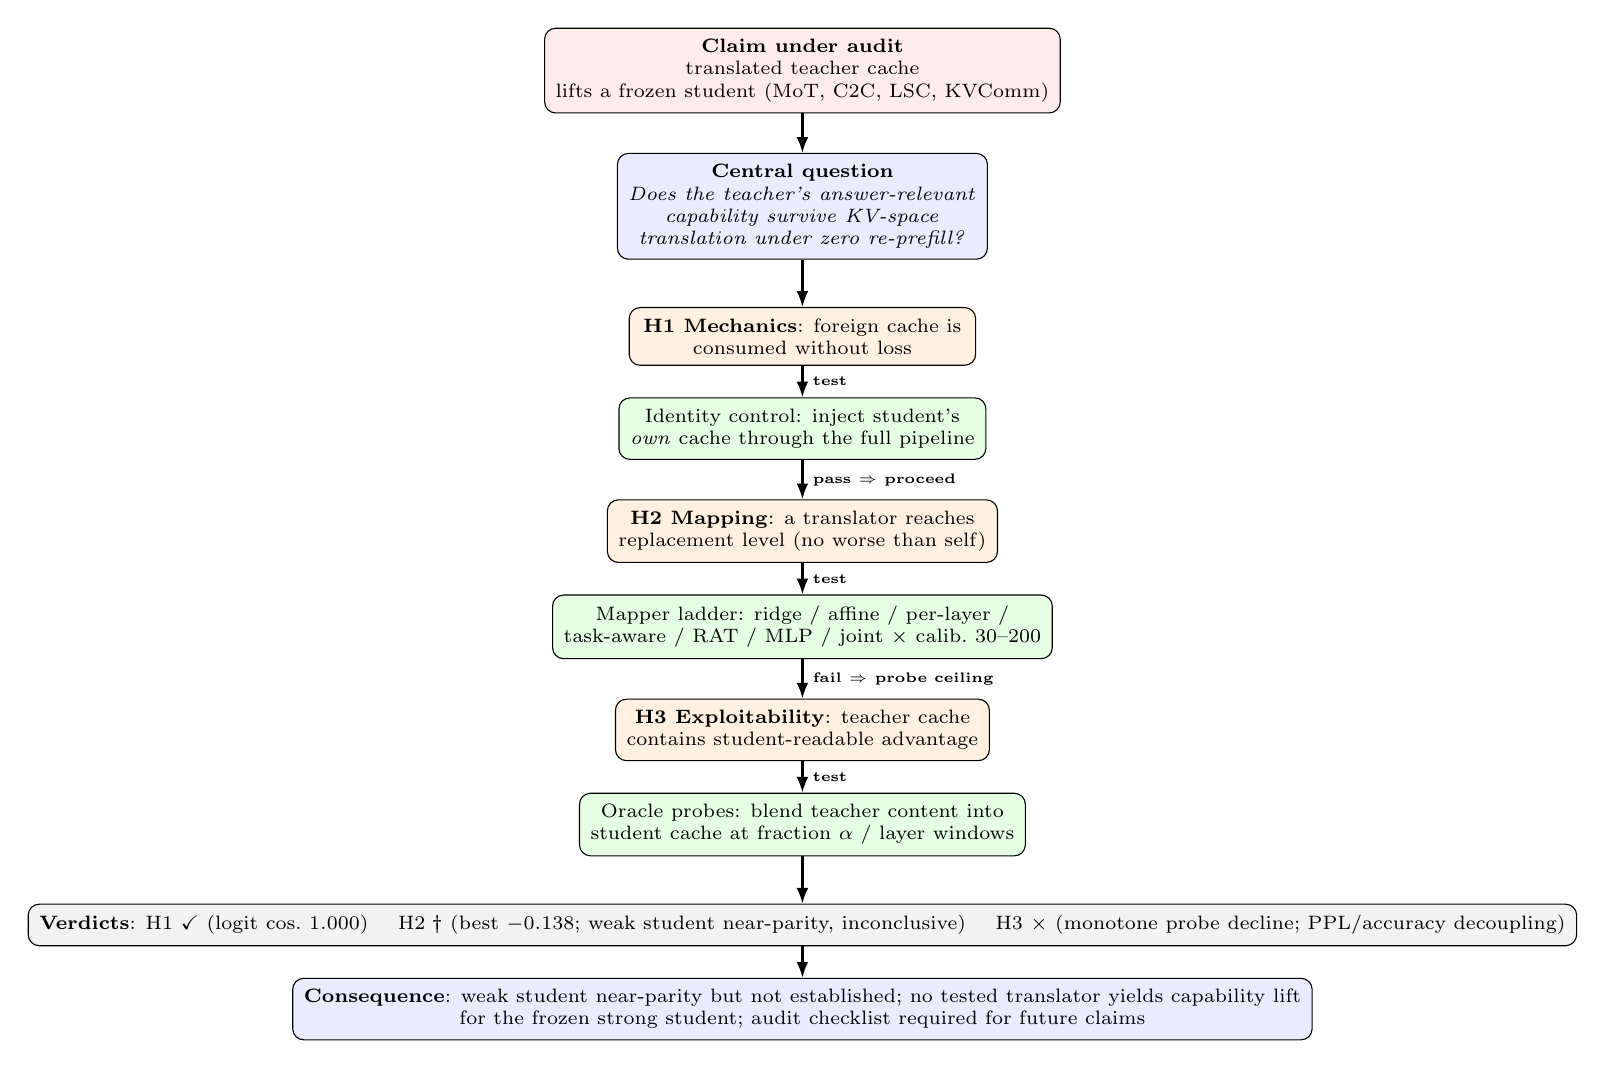
\begin{tikzpicture}[
  node distance=4mm and 6mm,
  box/.style={draw, rounded corners, align=center, inner sep=4pt,
              minimum width=34mm, font=\scriptsize},
  qbox/.style={box, fill=blue!8},
  hyp/.style={box, fill=orange!12, minimum width=44mm},
  inst/.style={box, fill=green!10, minimum width=44mm},
  verdict/.style={box, fill=gray!10, minimum width=44mm},
  gate/.style={diamond, draw, aspect=2.2, inner sep=1.5pt, font=\tiny\bfseries},
  arr/.style={-{Latex[length=2mm]}, thick},
  lab/.style={font=\tiny\bfseries},
]
\node[box, fill=red!8] (mot) {\textbf{Claim under audit}\\ translated teacher cache\\
lifts a frozen student (MoT, C2C, LSC, KVComm)};
\node[qbox, below=5mm of mot] (q) {\textbf{Central question}\\
\emph{Does the teacher's answer-relevant}\\
\emph{capability survive KV-space}\\
\emph{translation under zero re-prefill?}};
\node[hyp, below=6mm of q] (h1) {\textbf{H1 Mechanics}: foreign cache is\\
consumed without loss};
\node[inst, below=4mm of h1] (i1) {Identity control: inject student's\\
\emph{own} cache through the full pipeline};
\node[hyp, below=5mm of i1] (h2) {\textbf{H2 Mapping}: a translator reaches\\
replacement level (no worse than self)};
\node[inst, below=4mm of h2] (i2) {Mapper ladder: ridge / affine / per-layer /\\
task-aware / RAT / MLP / joint $\times$ calib.\ 30--200};
\node[hyp, below=5mm of i2] (h3) {\textbf{H3 Exploitability}: teacher cache\\
contains student-readable advantage};
\node[inst, below=4mm of h3] (i3) {Oracle probes: blend teacher content into\\
student cache at fraction $\alpha$ / layer windows};
\node[verdict, below=6mm of i3, minimum width=120mm] (v)
{\textbf{Verdicts}: H1 \checkmark\ (logit cos.\ $1.000$) \quad
H2 \textdagger\ (best $-0.138$; weak student near-parity, inconclusive) \quad
H3 $\times$ (monotone probe decline; PPL/accuracy decoupling)};
\node[box, fill=blue!8, below=4mm of v, minimum width=120mm] (c)
{\textbf{Consequence}: weak student near-parity but not established; no tested
translator yields capability lift\\ for the frozen strong student; audit
checklist required for future claims};
\draw[arr] (mot) -- (q);
\draw[arr] (q) -- (h1);
\draw[arr] (h1) -- node[lab, right] {test} (i1);
\draw[arr] (i1) -- node[lab, right] {pass $\Rightarrow$ proceed} (h2);
\draw[arr] (h2) -- node[lab, right] {test} (i2);
\draw[arr] (i2) -- node[lab, right] {fail $\Rightarrow$ probe ceiling} (h3);
\draw[arr] (h3) -- node[lab, right] {test} (i3);
\draw[arr] (i3) -- (v);
\draw[arr] (v) -- (c);
\end{tikzpicture}
\caption{The three-hypothesis audit as a decision pipeline. Each hypothesis
carries a dedicated instrument and a gate; H2's failure routes the audit to
H3's oracle probes, which probe exploitability without training a translator.}
\label{fig:framework}
\end{figure}

\section{A Survey of Cache-Level Communication Between Models}
\label{sec:survey}

We organize prior work into four lines and close each with the assumption it
leaves untested. Table~\ref{tab:related} summarizes the comparison.

\subsection{KV Reuse Within a Single Model}
Prompt caching, cache-augmented generation, and streaming attention reuse a
model's own cache across requests. Streaming attention identifies attention
sinks at early positions whose KV carries outsized attention
mass~\citep{streamingsink2023}. CacheGen compresses and streams a KV cache
across a network~\citep{cachegen2024}; CacheBlend fuses several cached
fragments with selective attention recomputation for
RAG~\citep{cacheblend2025}; KVSharer shares caches across layers that behave
dissimilarly~\citep{kvsharer2024}. These systems assume a single model on
both sides of the cache. The reuse question is therefore about storage and
attention cost, not about representation compatibility. Our audit inherits
their serving motivation but moves the mismatch to the model axis, where the
compatibility assumption breaks.

\subsection{Cross-Model Cache Translation}
The line closest to our audit translates caches between models. C2C proposes
direct cache-to-cache semantic communication with a depth-ratio layer
mapping~\citep{c2c2025}. LSC aligns caches through a shared latent space with
a cross-attention translator~\citep{lsc2026}. MoT combines gated translator
modules over depth-ratio channel windows with a Context Correction Loss that
aligns a replayed target trajectory with the native one, and reports the
strongest numbers to date: 51.0\% average closed-set QA accuracy at
Qwen2.5-7B$\to$0.5B and 96.3\% retention in long-context cache-augmented
generation~\citep{mot2026}. KVComm shares attention-ranked KV
layers~\citep{kvcomm2025}; Interlat communicates last-hidden-state
messages~\citep{interlat2025}; HCache restores caches from hidden-state
translations~\citep{hcache2025}. Two properties of this line matter for our
audit. First, its evaluations score the translated pipeline against the
student baseline, which conflates mechanics, mapping, and exploitability.
Second, its strongest variants do not operate under strict zero re-prefill:
MoT reconstructs the target-side cache by replaying the context through the
target model with source-guided sparse attention, so the reported quality
includes a correction pass that a cold-start deployment would not get. A naive
target-side replay pass does not by itself recover the strong student
(Appendix~\ref{app:replay}), so MoT's gains cannot be attributed to replay
alone. Our audit holds the zero-re-prefill constraint fixed and asks what a
translator alone can deliver. Our numbers sit far below the 73--98\% retention that
recent work reports for the same idea. Three protocol differences separate
the claims: those results do not hold strict zero re-prefill (they replay or
correct on the target side), they evaluate on a shared calibration/evaluation
split rather than a disjoint one, and they use different model pairs. Under
the strict regime, we measure gold-probability changes of $-0.25$ to $-0.30$
for the strong student; the gap is a property of the regime, not a
contradiction of those results.

\subsection{Cross-Model Representation Alignment}
A separate line asks whether two trained networks' representations can be
aligned at all. Model stitching connects frozen networks with a learned
linear layer and shows that stitching quality varies sharply across training
runs and layers~\citep{stitching2021}. Relative representations replace
absolute coordinates with anchor-based similarity spaces and enable zero-shot
communication between encoders~\citep{relrep2022}. The Platonic Representation
Hypothesis argues that representations converge across models up to linear
transform~\citep{platonic2024}, with refinements and proofs
following~\citep{aristotelian2026,perfectplatonic2025}. vec2vec translates
embeddings between models without paired data by exploiting this shared
geometry~\citep{vec2vec2025}. These results motivate the hypothesis that a
linear map between cache spaces should exist. Our results qualify the
conclusion for caches: the convergence evidence comes from pooled embedding
spaces, while a cache is a per-layer, per-head, position-indexed state whose
student-relevant content is not determined by its teacher counterpart
(Section~\ref{sec:why}).

\subsection{Frozen-Model Controllability}
Work on steering shows that a frozen model's behavior can be moved by
injecting activations: task vectors compress in-context learning into a
single mid-layer activation~\citep{taskvectors2023}; activation steering adds
behavioral directions to the residual stream; gist tokens compress prompts
into a few virtual tokens~\citep{gist2023}. The tuned lens reads intermediate
layers through per-layer affine probes~\citep{tunedlens2023}, and the FFN-as-
memory view assigns the factual capacity of a model to its feed-forward
weights~\citep{ffnmemory2021}. This line supports the intuition that a frozen
student can absorb injected information, which makes the H3 null result
informative rather than tautological: the failure is not that frozen students
cannot be steered. It is that, in our tested teacher--student regime, raw KV
translation does not deliver a usable steering signal to the frozen student.
More transferable control signals may be easier to access in residual-stream
directions or task-vector representations than in per-head KV entries.

\subsection{What the Survey Does Not Establish}
Across the four lines, no work (i) separates mechanics from mapping from
exploitability, (ii) injects the student's own cache as an identity control,
(iii) reports accuracy at matched perplexity, or (iv) bounds exploitability
with an oracle that requires no training. The claims of the translation line
therefore rest on pipelines whose components have never been isolated. The
audit below supplies the missing instruments.

\begin{table}[t]
\centering
\small
\caption{Cache-translation and adjacent work, organized by what is
translated and what is held fixed. ``Replay'' marks methods whose reported
quality includes a target-side correction pass over the context; our audit
holds strict zero re-prefill. No cited evaluation isolates mechanics with an
identity injection or reports accuracy at matched perplexity; MoT's
injection-window ablations are the closest antecedent
(Section~\ref{sec:survey}).}
\label{tab:related}
\begin{tabular}{p{2.6cm}p{2.2cm}p{2.4cm}p{1.6cm}p{3.4cm}}
\toprule
Work & What moves & Alignment & Replay & Unexamined assumption \\
\midrule
C2C~\citep{c2c2025} & Full KV & depth-ratio layers & no & a linear map per
channel suffices \\
LSC~\citep{lsc2026} & KV via shared latent & learned latent space & no &
one latent space fits all layers \\
MoT~\citep{mot2026} & KV windows & gated translators & yes (sparse) &
pipeline delta $\neq$ translation value \\
KVComm~\citep{kvcomm2025} & selected KV layers & attention ranking & no &
ranked layers carry the signal \\
Interlat~\citep{interlat2025} & last hidden state & latent message & no &
the last layer summarizes the cache \\
HCache~\citep{hcache2025} & hidden states & translator & no & states
determine caches \\
\midrule
This paper & full cache (zero re-prefill) & seven families incl.\ RAT & no &
\emph{identity-controlled evaluation} + diagnostic probes \\
\bottomrule
\end{tabular}
\end{table}

\section{The Three-Hypothesis Audit Framework}
\label{sec:framework}

\subsection{Setup}
Let a teacher $T$ prefill a context $x$ and form a cache
$C_T(x) = \{K^T_\ell, V^T_\ell\}_{\ell=1}^{L_T}$ with $L_T$ layers, $H$ KV
heads, and head dimension $d$. A translator $g_\theta$ maps it to
$\widehat{C}_S(x)$ in the space of a student $S$ with $L_S$ layers. The
student then answers a query $q$ with only the query tokens as input,
$\hat{y} = S(q \mid \widehat{C}_S(x))$, under strict zero re-prefill: the
context never enters the student's forward pass. Three references anchor the
audit. \emph{Student self-prefill} $S(q \mid C_S(x))$ is the baseline the
handoff must not degrade. \emph{Identity injection} feeds $C_S(x)$ itself
through the injection pipeline; it isolates mechanics from mapping.
\emph{Teacher full} $T(q \mid C_T(x))$ is the capability upper bound. We
measure answer quality by the gold-letter probability $\gold$, accuracy, and
the change $\chg = \gold(\text{handoff}) - \gold(\text{student self})$, with
95\% bootstrap intervals and sign-flip permutation tests; perplexity over the
scoring suffix is recorded but never accepted as evidence of capability
(Section~\ref{sec:decoupling}).

\subsection{Hypotheses, Instruments, Gates}
Figure~\ref{fig:framework} states the three hypotheses with their instruments
and gates. \textbf{H1}: the identity injection matches the student's own
prefill per sample (gate: mean logit cosine $= 1$ within float tolerance).
\textbf{H2}: some $g_\theta$ in the audited family reaches replacement level
(gate: the CI lower bound of gold CHG is above a small tolerance $-\epsilon$; a
stricter \emph{gain} gate additionally requires the CI lower bound $> 0$).
Replacement asks only that the student is not degraded; gain asks that the
teacher's cache provides a measurable lift. We fix $\epsilon = 0.02$ gold
probability before evaluation---about $4\%$ relative to the $0.503$ student
baseline, a practical serving tolerance---making the replacement gate a
standard non-inferiority test of $H_0\colon \chg \le -\epsilon$ against
$H_1\colon \chg > -\epsilon$; unlike a naive significance test, it does not
additionally require the point estimate to be non-negative. \textbf{H3}: the teacher's cache contains student-readable
advantage (gate: some oracle probe configuration with teacher content
improves over the student's own cache). H3's probe is decisive because it
does not depend on training a translator; it directly measures what a frozen
student can extract from teacher-cache content under the most favorable
mixing.

\section{Audit Methodology}
\label{sec:method}

\subsection{Identity Control}
At evaluation time we capture the student's own cache over the context
(allowed in calibration and probe stages), feed it through the same mapper
interface, cache construction, position handling, and scoring path as a
translated cache, and score. Any deviation from the student's own prefill is
mechanics loss. This is the control that prior evaluations omit.

\subsection{Disjoint Splits, Unified Prompts, and Honest Counters}
Mapper calibration and evaluation draws are disjoint samples of the same
distribution (HellaSwag and ARC-Challenge, shuffled then split). All methods
share one token-level prompt format, so the only difference between the
handoff and the student baseline is where the context representation comes
from. Zero-prefill counters read the actual cache length before and after the
scoring forward pass rather than trusting bookkeeping, and the scoring pass
uses an isolated cache because the deployed transformers version mutates a
cache even under \texttt{use\_cache=False}, which silently pollutes
co-located measurements.

\subsection{Mapper Ladder}
We audit seven families under one interface. \textbf{Ridge (per-head)}: a
$128\times128$ ridge map per student layer and head with Gram aggregation
over variable-length calibration samples. \textbf{Affine (per-head)}: the
same with mean centering and an intercept, fit in closed form over
concatenated calibration samples. \textbf{Affine (per-layer)}: heads merged
into rows, eight times fewer parameters. \textbf{Task-aware}: ridge
initialization plus a bounded task fine-tune that mixes reconstruction with
gold-answer cross-entropy (weight $\beta{=}0.3$) under a diagonal
parameterization with a per-layer bounded gate. \textbf{RAT
(residual-anchored translator)}: an architecture-derived map
\begin{equation}
W^{(s,h)} \;=\; \bigl[\,\pi(W^{S,h}_V)\;R\;\pi(W^{T,h}_V)\,\bigr]^{\!\top},
\qquad
R \;=\; \arg\min_R \; \|E_T R - E_S\|_F^2 + \lambda \|R\|_F^2,
\end{equation}
where $W^{T,h}_V$ and $W^{S,h}_V$ are the two models' own value projections
at the aligned layer pair, $\pi(\cdot)$ is the pseudo-inverse pullback from a
head's value space to the residual stream, and $R$ aligns the two residual
streams through the shared 151{,}936-token embedding matrices, which both
Qwen3 models ship. A closed-form rank-$r$ correction fits the calibration
residual on top of the analytic core, a Hungarian matching on head covariance
profiles replaces the identity head correspondence, and the sink position
(position 0) is overwritten with the student's calibration statistics because
its translated value is a PPL catastrophe (Section~\ref{sec:ratresults}).
\textbf{Joint MLP (over-parameterized)}: for each student layer, a
two-hidden-layer MLP with width $256$ maps the concatenation of all aligned
teacher layers and all KV heads at a position to all student heads, giving
about $37$M parameters across K and V, five times the per-head affine family;
it is trained on the calibration split by Adam for $300$ epochs.
Keys follow the same construction on $W_K$. Every family is evaluated at
calibration budgets 30 and 200 with disjoint evaluation samples
($n{=}30$ and $n{=}63$ respectively).

\subsection{Oracle Probes}
The probes assume an oracle that no training can beat: they hand the student
its \emph{own} cache and mix in teacher content at a controlled budget.
\textbf{Fraction probe}: $\alpha\widehat{C}_S + (1-\alpha)C_S$ for
$\alpha \in \{0.25, 0.5, 0.75\}$ with $\alpha{=}0$ the student's own cache.
\textbf{Window probe}: translated content in only the bottom, middle, or top
third of student layers, student content elsewhere. Because every
configuration keeps the student's own cache dominant or localized, any
improvement over $\alpha{=}0$ would indicate exploitable teacher-cache
content; monotone degradation under the tested translators rules out
exploitable content in this regime. Probes are
flagged non-deployable (they require the student's own prefill) and exist
only as measurement instruments.

\subsection{Pairs, Data, and Protocol Discipline}
Primary pair: Qwen3-4B (36 layers, hidden 2560) $\to$ Qwen3-1.7B (28 layers,
hidden 2048); contrast pair: $\to$ Qwen3-0.6B (hidden 1024); scale-extended
pair: Qwen3-8B (36 layers, hidden 4096) $\to$ 1.7B and 0.6B. All share the
same tokenizer, vocabulary, $H{=}8$ KV heads, $d{=}128$, and RoPE base
$10^6$. Every run records its git commit and protocol version in its
artifacts; every number below is read directly from a recorded run.
We use multiple-choice QA deliberately: it gives a gold-probability control
(the correct option's log-probability is comparable across cache states),
and it makes disjoint calibration/evaluation splits enforceable without
leakage. We also run the audit on a long-context needle
multiple-choice check (Section~\ref{sec:results}); task diversity beyond this
format remains future work.

\section{Results}
\label{sec:results}

\subsection{H1 Passes: Mechanics Is Not the Failure Mode}
The identity control reproduces the student's own prefill exactly: per-sample
logit cosine $1.000$, gold CHG $+0.0001$ $[-0.0006, +0.0009]$, $n{=}30$. The
injection pipeline, cache construction, GQA head handling, and position
accounting are therefore correct, and every subsequent gap is attributable to
the translation itself. The same control verified the disk-persistence path:
a cold-start evaluation that loads a persisted cache and mapper parameters
reproduces the offline run bit-for-bit.

The identity control also fixes the perplexity protocol used below. Injected
caches are scored on the suffix conditioned on the cache, so the
identity-injection PPL ($21.2$) is the student's own suffix PPL and matches the
native suffix distribution by construction. The student self-prefill row of
Table~\ref{tab:main} reports a different quantity---the native loss averaged
over the full context and suffix in one pass---so its value ($25.4$) is not
expected to equal the injected-cache PPL. The H1 identity criterion is defined
on the answer-scoring logits, where the two paths agree to float tolerance.

\subsection{H2 Fails for the Strong Student; the Weak-Student Result Is Inconclusive}
\begin{figure}[t]
\centering

\includegraphics[width=0.72\textwidth]{figures/fig2_mapper_landscape.pdf}
\caption{The mapper landscape for Qwen3-4B$\to$1.7B under the unified audit
protocol: gold-probability CHG over the student's own prefill, with 95\%
bootstrap CIs. No family reaches zero; calibration budget moves affine mapping by only
$0.005$ on a fixed evaluation set; the architecture-anchored RAT, the
nonlinear MLP, and the over-parameterized joint MLP sit inside the same band.}
\label{fig:landscape}
\end{figure}

\begin{table}[t]
\centering
\caption{Main audit results. Acc/gold/PPL: answer accuracy,
gold-letter probability, and perplexity of the scoring suffix for
the translated cache (kv-both). PPL entries for translated and identity
caches score only the suffix conditioned on the injected cache; the student
self-prefill row is the native loss over the full context and suffix in one
pass and is not directly comparable (the identity-injection value is the
student's suffix PPL). CHG is the gold-probability change
over the student's own prefill with 95\% bootstrap CIs. Pairs:
Qwen3-4B$\to$1.7B unless noted; rows marked 8B use the Qwen3-8B
teacher. $n_{\mathrm{eval}}$ is the evaluation sample count (tail
protocol rows use a fixed evaluation set of 100). All runs use
disjoint calibration/evaluation splits and the unified prompt
format.}
\label{tab:main}
\small
\begin{tabular}{lcccc}
\toprule
Configuration & Acc / Gold / PPL & Gold CHG [95\% CI] & $n_{\mathrm{eval}}$ \\
\midrule
Identity control (self-kv), 1.7B & 0.500 / 0.503 / 21.2 & $+0.000$ [$-0.001, +0.001$] & 30 \\
Student self-prefill, 1.7B & 0.500 / 0.503 / 25.4 & -- & 30 \\
Teacher (full prefill), 1.7B & 0.767 / 0.693 / -- & -- & 30 \\
Native average, 1.7B & 0.167 / 0.169 / 536082.5 & $-0.334$ [$-0.508, -0.154$] & 30 \\
Ridge per-head, c=30, 1.7B & 0.200 / 0.207 / 88.5 & $-0.296$ [$-0.479, -0.121$] & 30 \\
Ridge per-head, c=500, 8B$\to$1.7B & 0.310 / 0.288 / 146.1 & $-0.224$ [$-0.320, -0.123$] & 100 \\
Affine per-head, c=30, 1.7B & 0.367 / 0.365 / 46.1 & $-0.138$ [$-0.317, +0.029$] & 30 \\
Affine per-head, c=200, 1.7B & 0.254 / 0.258 / 56.4 & $-0.239$ [$-0.354, -0.134$] & 63 \\
Affine per-layer, c=200, 1.7B & 0.206 / 0.222 / 81441.1 & $-0.275$ [$-0.407, -0.140$] & 63 \\
Task-aware, c=200, 1.7B & 0.270 / 0.280 / 142.1 & $-0.216$ [$-0.336, -0.105$] & 63 \\
RAT, c=30, 1.7B & 0.233 / 0.235 / 501.6 & $-0.268$ [$-0.440, -0.092$] & 30 \\
RAT, c=200, 1.7B & 0.238 / 0.276 / 1008.2 & $-0.221$ [$-0.340, -0.104$] & 63 \\
RAT no-anchor rank-32, c=30, 1.7B & 0.267 / 0.280 / 23.7 & $-0.223$ [$-0.367, -0.088$] & 30 \\
Joint MLP, c=30 (3 seeds), 1.7B & 0.189 / 0.219 / 28.9 & $-0.30$ to $-0.26$ & 30 \\
Affine per-head, c=200, 4B$\to$0.6B & 0.302 / 0.283 / 71.8 & $+0.010$ [$-0.081, +0.102$] & 63 \\
Affine per-head, c=30, 8B$\to$0.6B & 0.270 / 0.269 / 99.0 & $-0.023$ [$-0.104, +0.064$] & 100 \\
RAT, c=200, 4B$\to$0.6B & 0.206 / 0.232 / 790.0 & $-0.041$ [$-0.120, +0.038$] & 63 \\
Affine per-head, c=30, long-context & 0.233 / 0.232 / 6554.1 & $-0.285$ [$-0.534, -0.025$] & 30 \\
\bottomrule
\end{tabular}
\end{table}

Figure~\ref{fig:landscape} and Table~\ref{tab:main} give the landscape.
Centering is the single biggest gain: per-head ridge ($-0.296$) drops to
per-head affine ($-0.138$), roughly halving the deficit. The teacher and
student value distributions differ in location and scale before they differ
in content, which is exactly what the measured norm ratios say ($1.58\times$
for keys, $7.44\times$ for values). The calibration budget, by contrast,
buys nothing. Holding the evaluation set fixed ($n{=}100$) and sweeping the
calibration budget, affine mapping keeps CHG
inside $[-0.257, -0.238]$: $-0.251$ at $c{=}10$, $-0.249$ at $c{=}30$,
$-0.238$ at $c{=}60$, $-0.257$ at $c{=}100$, and $-0.244$ for the full
calibration pool (budgets beyond the pool size saturate and reproduce the
full-pool result exactly), a spread of $0.019$. The mapper has converged, and
more data cannot close a gap that is set by the information content of the
translated cache rather than by estimation variance. Refitting the headline
mapper on five independent calibration draws, with the evaluation set fixed,
moves gold CHG within $[-0.292, -0.249]$ (SD $\approx 0.018$): the verdict
is not an artifact of one calibration draw. Structure and function
class change little either: per-layer merging ($-0.275$), task-aware
fine-tuning ($-0.216$), RAT ($-0.221$ to $-0.268$), and a per-head MLP mapper
with two GELU layers (CHG $-0.39$ to $-0.26$ at $c{=}30$ and $-0.26$ to
$-0.23$ at $c{=}200$ across independent trainings) all sit inside the same
band. Nonlinearity does not help. An over-parameterized joint
mapper ($\sim$$37$M parameters) that reads all teacher layers and all KV heads
also fails: across three training seeds its CHG spans $-0.26$ to $-0.30$ with
accuracy $0.189$, even though it reconstructs a fluent cache (PPL $28.9$
versus $25.4$ for the student). The strong student never
approaches its own prefill ($0.503$); the best mapper reaches $0.365$. Scaling
the teacher to 8B under the same protocol does not change the verdict:
self-injection remains an identity (logit cosine $0.99998$) and the ridge
mapper reaches CHG $-0.224$ $[-0.320, -0.123]$ at $c{=}500$, so H2's failure
is robust to teacher scale. The
weak 0.6B student tells the opposite story. Affine at $c{=}200$ gives a
near-parity point estimate $+0.010$ $[-0.081, +0.102]$, and 8B$\to$0.6B gives
$-0.023$ $[-0.104, +0.064]$; both intervals include zero, but both lower
bounds fall below the pre-specified replacement margin $-\epsilon=-0.02$, so
non-inferiority is not established at these sample sizes.

The failure is not specific to short commonsense contexts. On a long-context
needle-in-a-haystack multiple-choice task (contexts of about $1024$ tokens,
$n{=}30$), where the teacher answers from a retrievable fact ($0.733$ accuracy
versus the student's $0.533$), affine translation again fails: accuracy drops
to $0.233$ with gold CHG $-0.285$ $[-0.534, -0.025]$, while identity injection
remains exact (CHG $+0.000$ $[-0.001, +0.001]$). The deficit therefore tracks
the translation regime rather than the context length or task format.

Cross-architecture checks relax the one-family scope
(Table~\ref{tab:crossarch}). Replacing the Qwen3 student with five models from
other families---Llama-3.2-1B and 3B, Gemma-2-2B, Gemma-3-1B, and
Qwen2.5-1.5B, spanning one to eight KV heads and head dimensions $64$ to
$256$---mechanics still hold (self-kv CHG within $\pm0.001$) and translation
never recovers the teacher's $0.691$ gold. Four students are harmed (CHG
$-0.009$ to $-0.157$); the weakest, near-chance student (Llama-3.2-1B) is
non-inferior but gains nothing. Head groups are mean-pooled and head
dimensions projected by the rectangular mapper; because the models tokenize
independently, calibration pairs are matched position-by-position, so we read
these as mechanism and replacement checks rather than fine-grained capability
measurements. To address the tokenization confound directly, a token-aligned
variant maps each student token to the teacher token with maximum character
overlap before fitting and gives the same verdict on genuine cross-tokenizer
pairs (Llama-3.2-3B: CHG $-0.024$ $[-0.047,-0.004]$; Gemma-3-1B: $-0.073$
$[-0.134,-0.021]$), so the negative result is not an artifact of independent
tokenization; Qwen2.5 shares the Qwen tokenizer, making alignment a no-op
there.

\begin{table}[t]
\centering
\caption{Cross-architecture robustness checks. Qwen3-4B teacher to non-Qwen
and Qwen2.5 students under the within-family protocol (HellaSwag / ARC,
$c{=}30$, $n{=}100$); identity injection passes in every row (self-kv CHG
within $\pm0.001$). ``KV h/d'' gives the student's KV heads and head
dimension; the rectangular mapper mean-pools head groups and projects the
head dimension. Rows marked ``token-aligned'' align teacher KV to student token
positions by character overlap before fitting. No row recovers the teacher's
gold probability ($0.691$).}
\label{tab:crossarch}
\footnotesize
\begin{tabular}{lcccc}
\toprule
Student & KV h/d & Student acc / gold & Translated acc / gold & Gold CHG [95\% CI] \\
\midrule
Llama-3.2-1B & 8/64 & 0.300 / 0.254 & 0.260 / 0.254 & $+0.000$ [$-0.012, +0.012$] \\
Gemma-2-2B & 4/256 & 0.270 / 0.257 & 0.220 / 0.248 & $-0.009$ [$-0.020, +0.002$] \\
Llama-3.2-3B & 8/128 & 0.390 / 0.281 & 0.200 / 0.237 & $-0.044$ [$-0.073, -0.013$] \\
Qwen2.5-1.5B & 2/128 & 0.400 / 0.385 & 0.200 / 0.228 & $-0.157$ [$-0.209, -0.106$] \\
Gemma-3-1B & 1/256 & 0.360 / 0.318 & 0.270 / 0.257 & $-0.061$ [$-0.135, +0.008$] \\
Llama-3.2-3B (token-aligned) & 8/128 & 0.390 / 0.281 & 0.280 / 0.257 & $-0.024$ [$-0.047, -0.004$] \\
Gemma-3-1B (token-aligned) & 1/256 & 0.360 / 0.318 & 0.250 / 0.245 & $-0.073$ [$-0.134, -0.021$] \\
\bottomrule
\end{tabular}
\end{table}

\subsection{RAT Component Ablations Separate Fluency From Capability}
\label{sec:ratresults}
RAT ablations attribute the failure inside the architecture-anchored design.
Removing the sink override explodes suffix perplexity to $2.7\times10^{5}$:
the translated position-0 entry, which carries outsized attention mass, is a
catastrophe unless overwritten with the student's own statistics. Removing
the analytic core and raising the correction rank to 32 \emph{repairs
fluency}: PPL drops to $23.7$, within $2.5$ of the identity control. Accuracy
stays at $0.267$. The analytic core's min-norm pullback is harmful on real
models, and more importantly, fluency recovery does not touch the answer
deficit. The cache can be made to look right to the language-modeling
objective without becoming right for the task. RAT's role in the audit is to
rule out the objection that the failure is an artifact of insufficiently
architecture-aware translation.

\subsection{H3: No Teacher-Content Probe Improves on the Student}
\begin{figure}[t]
\centering

\includegraphics[width=0.95\textwidth]{figures/fig3_oracle_probes.pdf}
\caption{Oracle probes on Qwen3-4B$\to$1.7B. Left: blending teacher-cache
content into the student's own cache (RAT translator) degrades gold
probability and accuracy monotonically in the teacher fraction $\alpha$;
$\alpha{=}0$ is the student's own cache. Right: per-octant window injection
(affine translator; octant $0$ = bottom eighth of student layers); only
layers $10$--$13$ (octant $3$) are clearly harmful, while the top three
octants are indistinguishable from the student.}
\label{fig:probes}
\end{figure}

The probes answer H3 without training anything
(Figure~\ref{fig:probes}). With $75\%$ student cache and $25\%$ teacher
content, gold probability already falls from $0.5031$ to $0.3798$; the decay
is monotone through $\alpha{=}0.75$. Window injection localizes the damage:
replacing the top third of layers is indistinguishable from the student
($0.5022$ versus $0.5031$), while the middle and bottom thirds are strongly
harmful ($0.2653$, $0.2242$). This is a sensitivity profile: the student's
behavior is substantially more sensitive to teacher-cache intervention in
early and middle layers than in the top third. It does not by itself locate
where the answer is routed; early and middle layers may also be more sensitive
to off-manifold perturbations. An eight-way octant sweep ($n{=}30$)
localizes the sensitive band: among the eight eighths of student layers, only
layers 10--13 have a gold-probability interval excluding zero (CHG $-0.186$
$[-0.322, -0.060]$, gold $0.317$ versus $0.503$), while the top three eighths
are statistically indistinguishable from the student (CHG $-0.011$ to
$+0.020$).
The probes were run with two translators: the RAT mapper reported above and
the affine mapper (the best in the ladder, gold $0.365$). Both show the same
monotone decline. With affine at $\alpha{=}0.25$, gold CHG is $-0.086$
(CI $[-0.18, +0.00]$); at $\alpha{=}0.75$, $-0.211$ (CI $[-0.41, -0.02]$).
The verdict is robust to translator quality: even the best available mapper
produces content that the frozen student cannot exploit.

Direct native-cache injection provides an additional negative control:
injecting the teacher's native
(norm-rescaled) cache entries directly degrades the student to $-0.334$
[$-0.508, -0.154$] ($n{=}30$), and the norm-rescaled native ablation
replicates under the fixed-evaluation protocol ($-0.266$ [$-0.363, -0.168$]
at $c{=}30$ and $-0.251$ [$-0.351, -0.152$] at $c{=}200$, $n{=}100$), so
even untranslated teacher content in student coordinates does not help: the
harm is not an artifact of any particular mapper.

\subsection{Perplexity and Accuracy Decouple}
\label{sec:decoupling}
\begin{figure}[t]
\centering

\includegraphics[width=0.6\textwidth]{figures/fig4_ppl_acc_decoupling.pdf}
\caption{Perplexity over the scoring suffix versus accuracy across all
methods and runs (log scale). The identity control and the student sit at
low PPL and high accuracy; translated caches span two regimes; the
best-reconstructed cache (PPL 23.7) remains 23 accuracy points below the
student.}
\label{fig:decoupling}
\end{figure}

Figure~\ref{fig:decoupling} plots perplexity against accuracy for every
method and run. The identity control and the student occupy the top-left
regime. Translated caches populate a broad band, including a point with
near-native perplexity and a 23-point accuracy deficit. Native injection
sits at extreme perplexity ($5.4\times10^{5}$) with low accuracy. Perplexity
measures whether the cache permits fluent continuation; accuracy measures
whether the cache supports the task. The two dissociate, so perplexity
cannot serve as evidence of translation quality, a practice that appears in
the serving literature because perplexity is cheap.

\subsection{Channel Asymmetry}
Channel ablations at $c{=}30$ rank value-only ($0.367$) above key-only
($0.300$) above both ($0.200$) on accuracy, while perplexity orders them in
reverse ($88$ versus $253$ versus $1.8\times10^{7}$). Mapping keys repairs
fluency and damages routing: the mapped keys steer attention to plausible
but task-irrelevant positions. We report the asymmetry as a finding and
leave the mechanism open. One hypothesis consistent with the asymmetry:
mapped keys steer attention routing while mapped values carry content, so key
errors misroute a fluent read while value errors corrupt it audibly.

\section{Why Translation Fails: An Architectural Analysis}
\label{sec:why}

We read this section as an architectural explanation of the audit's
verdicts, not an impossibility result: the argument is per-head and
does not cover exploit paths that read the full multi-head,
multi-layer cache (Section~\ref{sec:limitations}).

The audit's verdicts fit the architecture. A cache entry is a linear
projection $W_V h$ of a residual-stream state $h$. Translation must recover
$h$ from $V$, move it across the residual-space gap ($2560$ to $2048$), and
re-project. Two facts bound the recovery. First, the pullback
$\pi(W_V)V$ returns only the row-space component of $h$; the component
orthogonal to $W_V$'s rows, which can dominate a $2560$-dimensional state
observed through a $128$-dimensional head, is invisible in that head's value
entry, so the per-head student value is underdetermined by its teacher
counterpart. The
student's corresponding value $W_V^S R\, h$ depends on that invisible
component, so the per-head student value is not determined by the per-head teacher value alone: the mapping task is
intrinsically underdetermined, and a learned translator can at best track the
conditional mean. The mapper-fitting view quantifies this: on held-out
calibration contexts, the fitted per-head affine mapper recovers student key
states (mean $R^2 = +0.81$) but only partially recovers value states (mean
$R^2 = +0.32$): roughly two-thirds of the value variance is not linearly
recoverable from the teacher's per-head entry. The unit is a held-out
calibration context: we fit on 20 contexts and score 10 disjoint held-out
contexts; each yields a per-(layer,head) $R^2$ between predicted and true
student states (pooled over token positions), and we report the mean over
heads, layers, and the 10 contexts. The repository's per-head ridge baseline
agrees on the same held-out contexts (pooled $R^2 = +0.92$ for keys, $+0.29$
for values). Second, the teacher's advantage over the student sits in its
parameters. FFN layers carry the model's factual
associations~\citep{ffnmemory2021}, and the capability gap between Qwen3-4B
and 1.7B is a gap in these parameters, which a cache does not transport. The
oracle probes make the consequence concrete: even with the student's own
cache holding $75\%$ of the mass, the teacher's $25\%$ contribution degrades
the answer. MoT's own design corroborates the analysis: its reported quality
includes a target-side replay with a correction loss, which is exactly the
upper-layer correction that strict zero re-prefill denies. Under a cold
start the translator's output is all the student gets, and that output shows
no measurable teacher advantage in our audit.

\section{Implications for Cache-Translation Research}
\label{sec:implications}

Any future cache-translation evaluation should ship three instruments:
\begin{itemize}
\item an \emph{identity control} that injects the student's own cache through
the full pipeline and must reproduce the student's own prefill;
\item a \emph{gold-probability metric} with bootstrap intervals and
permutation tests, reported as the change over the student's own prefill;
\item \emph{oracle probes} that blend teacher-cache content into the student
cache at controlled fractions and layer windows, bounding exploitability
without training anything.
\end{itemize}
Two gates apply to the metric: a replacement gate requires the bootstrap CI
lower bound above a pre-specified tolerance $-\epsilon$ (the point estimate
need not be non-negative), and a stricter
gain gate requires the CI lower bound above zero. A pipeline delta over a
student baseline is not evidence of translation, and a perplexity gain is not
evidence of capability. Each instrument costs one evaluation run and composes
with any serving stack.

For deployment, the weak student presents a near-parity regime rather than a
demonstrated capability transfer. At 0.6B, translated injection is
statistically indistinguishable from self-prefill
(4B$\to$0.6B: $+0.010$ $[-0.081,+0.102]$; 8B$\to$0.6B: $-0.023$
$[-0.104,+0.064]$), but neither interval clears the pre-specified
non-inferiority margin, so replacement-level service is not established, and
at near-chance absolute accuracy ($0.302$ versus $0.25$ random) this is not an
endorsement. Top-layer injection is harmless, which means a system that
must spend translation capacity can spend it there, though our probes also
show it buys nothing there. Whether a capacity boundary separates a
near-parity regime from failure is the question the 8B
and 0.6B pairs begin to answer, and the audit protocol is built to test it.
For strong students, cache translation is currently a net negative, and the
honest fallback is the text channel: the teacher's summary of the context
scores $0.367$ (gold $0.372$) against the student's $0.500$ (gold $0.503$)
full-text baseline,\footnote{Text-channel numbers come from the v12-era
in-run ablation ($n{=}30$, disjoint calibration/evaluation splits);
per-sample scores were not persisted for that run, so only aggregate
accuracy and gold probability are reported and no bootstrap CI is
available.} so compression loses less than translation does on the strong
student.

The survivable versions of the idea move work off the cache and onto the
weights or the replay: allow a target-side correction pass the way MoT does,
train student-side adapters, or translate through a shared latent space
anchored by task vectors instead of per-entry caches. Each option gives up
part of the cold-start guarantee, and each deserves a fresh identity control
before its delta gets attributed to translation.

\section{Limitations}
\label{sec:limitations}
Our audit is centered on one model family (Qwen3) with four scale pairs, plus
a cross-family check (five students, Table~\ref{tab:crossarch}) and HellaSwag /
ARC-Challenge and long-context needle tasks, with $n{=}30$--$100$ evaluation
samples per run; the CI widths reflect that. The cross-family check matches
positions after independent tokenization and its student is near chance, so it
establishes mechanism and replacement, not capability. The oracle probe bounds exploitability under linear blending and
three-layer windows; a nonlinear exploit path outside this family would not
be detected, though it would also need to survive the same measurement
protocol. RAT's analytic core assumes value projections are informative
pullbacks of the residual stream; the synthetic validation confirms the
mathematics, and the real-model failure is itself an audit finding. We did
not re-implement MoT's full replay pipeline; our claims concern the
zero-re-prefill regime that its predecessors and our deployment target
share. H2 is scoped to translators trainable from the disjoint calibration
budget we test ($\le 200$ examples), which includes the common linear and
nonlinear families and a $37$M-parameter joint MLP. The mapper-ladder results use a single seed per configuration. Because the
mapper fit is deterministic given its calibration draw, we bound
mapper-training variance directly: refitting the headline mapper on five
independent calibration draws with the evaluation set fixed moves gold CHG
within $[-0.292, -0.249]$ (per-draw SD $\approx 0.018$) --- inside the
per-run bootstrap intervals --- and identical configurations reproduce
results bit-for-bit. The gradient-trained per-head MLP is the exception: its
value is training-seed dependent, so we report it as a range (Section~\ref{sec:results});
every deterministic family reproduces exactly.

\section{Conclusion}
Cache translation promises to move a teacher's work into a smaller model,
and the audit separates that promise into three testable parts. The
mechanism holds up: an identity control reproduces the student's own prefill
exactly. The tested maps do not reach replacement: seven mapper families, a calibration ladder, and an
architecture-anchored translator all leave the strong student below its own
prefill, while the weak student's near-parity point estimate remains
inconclusive under the pre-specified margin. The map, moreover, is not where the
problem sits. No probe configuration delivers a student-readable advantage from the
teacher's cache, and a near-native-perplexity cache still fails the
task. The evidence is consistent with a weight-mediated advantage:
recovering the teacher's edge from raw KV states would take more than
the tested translators provide (scope limits in
Section~\ref{sec:limitations}). The audit framework is
packaged so that the next cache-translation claim can be checked in a single
run.

\bibliographystyle{plainnat}
\bibliography{references}

\appendix

\section{Reproducibility}
All numbers come from the \texttt{apcs} repository's recorded runs
(\texttt{reports/runs/*/inject-eval/}), each carrying its git commit,
protocol version, configuration, and per-sample scores. An independent
reproduction of the deterministic configurations---ridge, affine, per-layer,
task-aware, RAT, joint MLP, the calibration ladder, probes, octant windows,
and the cross-architecture checks---matches the recorded values within
$0.002$; the gradient-trained per-head MLP is seed-dependent and reported as
a range (Table~\ref{tab:main}). The held-out
reconstruction $R^2$ is produced by \texttt{scripts/measure\_reconstruction\_r2.py}
(output under \texttt{reports/reconstruction\_r2/}). The audit protocol
is implemented in \texttt{apcs.inference.evaluator} with the flags
\texttt{calib\_eval\_split}, \texttt{calib\_shuffle}, \texttt{probe\_mode},
and \texttt{native\_rescale}; mapper families live in \texttt{apcs.mapper}
(\texttt{math}, \texttt{joint}, \texttt{task\_aware}, \texttt{rat}, the
per-head MLP in \texttt{mlp}, the joint MLP in \texttt{joint\_mlp}, and the
cross-family rectangular map in \texttt{rect}); the
long-context needle task loader is \texttt{needle\_mcqa} in
\texttt{apcs.data.hf\_dataset};
persistence and the cold-start online phase in
\texttt{apcs.inference.kv\_store}. Unit tests cover the audit counters, the
store round-trip, and the mapper interface.

\section{Additional Measurements}
The teacher/student KV norm ratios are $1.58\times$ (keys) and $7.44\times$
(values), measured over 30 calibration contexts per layer. Norm rescaling of
the native cache repairs neither its perplexity ($5.4\times10^{5}$) nor its
accuracy, ruling out scale as the primary failure. The unified prompt
renders choices once; the earlier protocol rendered them twice for the
student baseline, which inflated the confidence-based deltas reported in our
own preliminary sweeps and motivated the unified format in the audit.


\section{Target-Side Replay Diagnostic}
\label{app:replay}
The audit holds strict zero re-prefill fixed, while MoT's reported quality
additionally includes a target-side replay with a Context Correction Loss. To
probe how much a replay pass alone contributes, we add a diagnostic that
re-reads the context through the student on top of the translated cache before
scoring; it is explicitly non-deployable because it violates zero re-prefill.
On Qwen3-4B$\to$1.7B (affine $c{=}30$, $n{=}100$), replay leaves accuracy at
$0.290$ and gold CHG at $-0.232$ $[-0.333, -0.136]$, statistically
indistinguishable from the no-replay result ($-0.249$) and far below the
student's own prefill ($0.520$, CHG $+0.000$). A naive replay pass therefore
does not recover the strong student; recovery requires either discarding the
translated cache (re-prefill) or the trained correction MoT uses. We do not
implement MoT's Context Correction Loss, so we cannot attribute its gains to
replay alone.

\end{document}
